\documentclass{article}
\usepackage{graphicx} % Required for inserting images
\usepackage{amsmath}
\usepackage{pgfplots}
\usepackage{tikz}
\usetikzlibrary{angles,quotes}
\usepackage{ amssymb }


\title{Remainder topics}
\author{Intro to Robotics}
\date{}

\begin{document}

\maketitle

\section{Torques and Forces on Joints}
Two type of joints -revolute and prismatic.\\
Revolute produces torque and prismatic produces force.\\\\
\textbf{Equation:} $\tau = {}^0J \hat{F}$ where,:\\
$\tau:$ is the vector of torques and forces for each joint\\
$\hat{F}: $ the unit forces\\\\
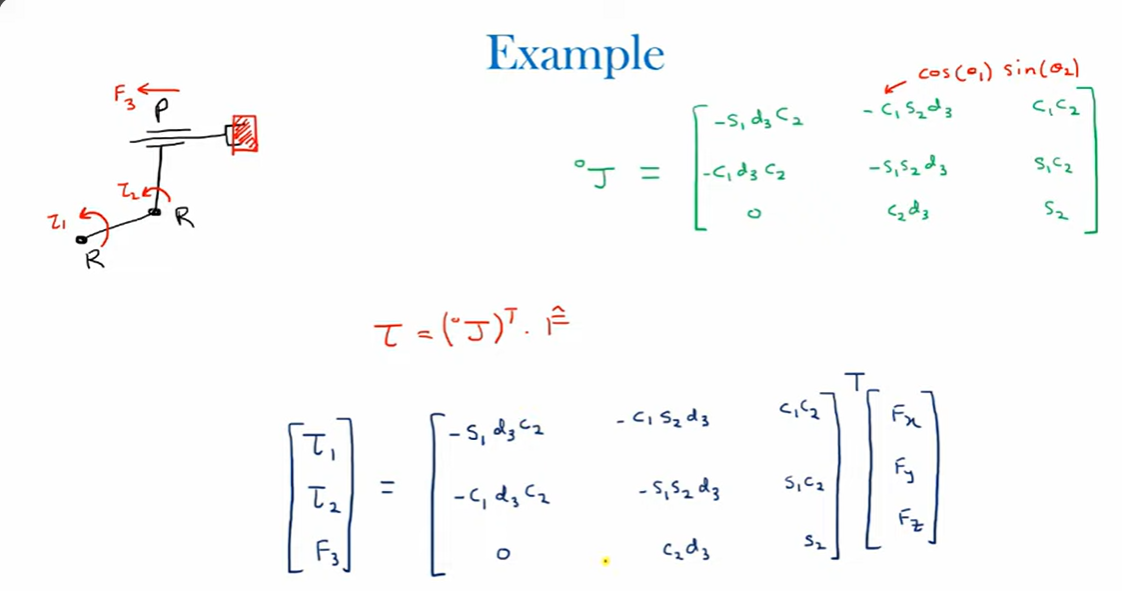
\includegraphics[width=10cm]{torques_forces_example.png}


\section{Lagrangian Mechanics (Torques and Forces)}
\textbf{Goal:} Find the torques or forces acting on a joint\\
$\mathcal{L}=$ kinetic(KE) $-$ potential(PE)\\
\begin{itemize}
    \item KE = $\frac{1}{2}mv^2$
    \item PE = $mgh$
    \item $\theta = position$
    \item $\dot{\theta} = velocity$
    \item R $\rightarrow$ torque (revolute)
    \item P $\rightarrow$ force (prismatic)
\end{itemize}

\subsection{Algorithm}
\begin{itemize}
    \item Robot manipulator $\rightarrow$ Position vector $(\theta)$
    \item Differentiate $\rightarrow$ velocity vector $(\dot{\theta})$
    \item KE = $\frac{1}{2}mv$, PE = $mgh$
    \item $\mathcal{L}$= KE - PE
    \item $\tau = \frac{d}{dt}(\frac{\partial \mathcal{L}}{\partial \dot{\theta}}) - \frac{\partial \mathcal{L}}{\partial \theta} - $[external forces/torques]$\theta$ \textbf{or F}
\end{itemize}

\subsection{Example}
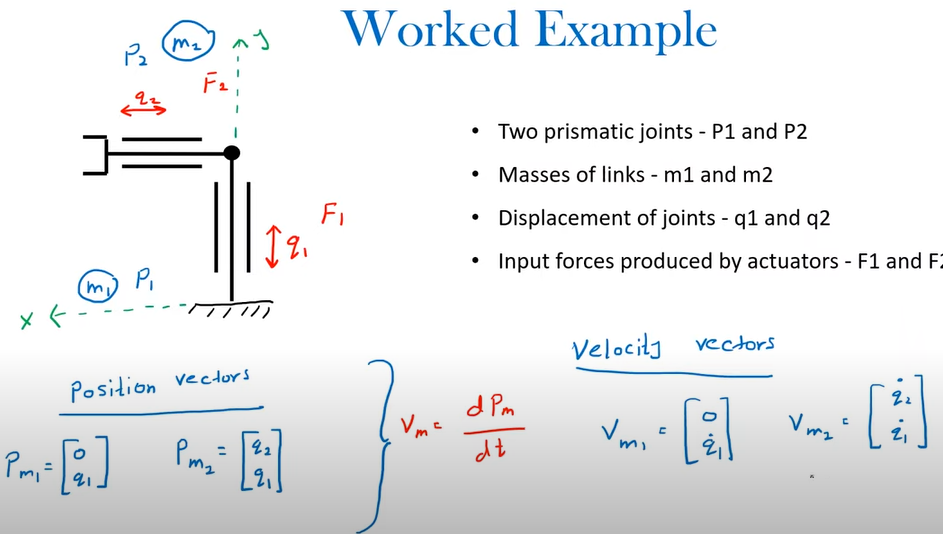
\includegraphics[width=10cm]{part1_lagrange.png}\\
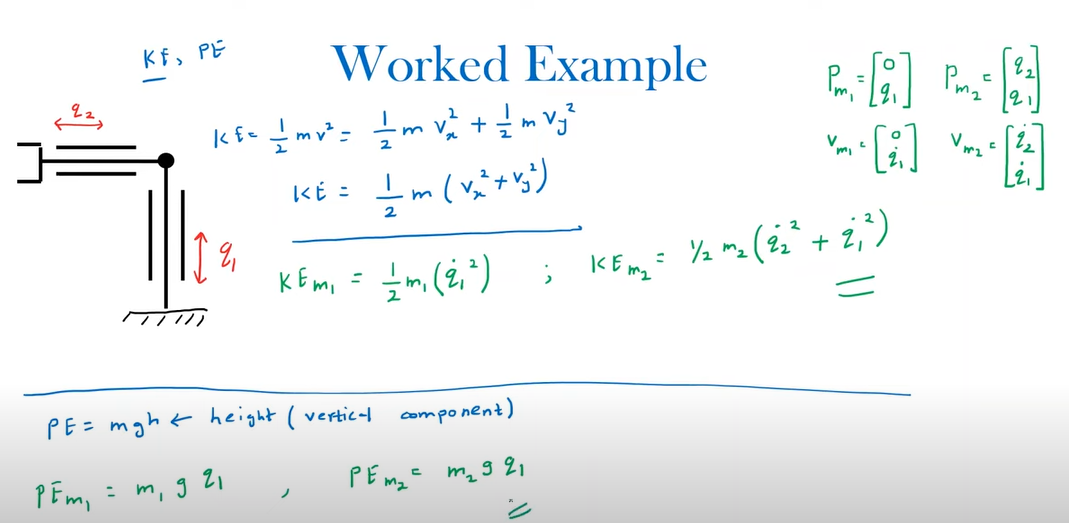
\includegraphics[width=10cm]{part2_lagrange.png}\\
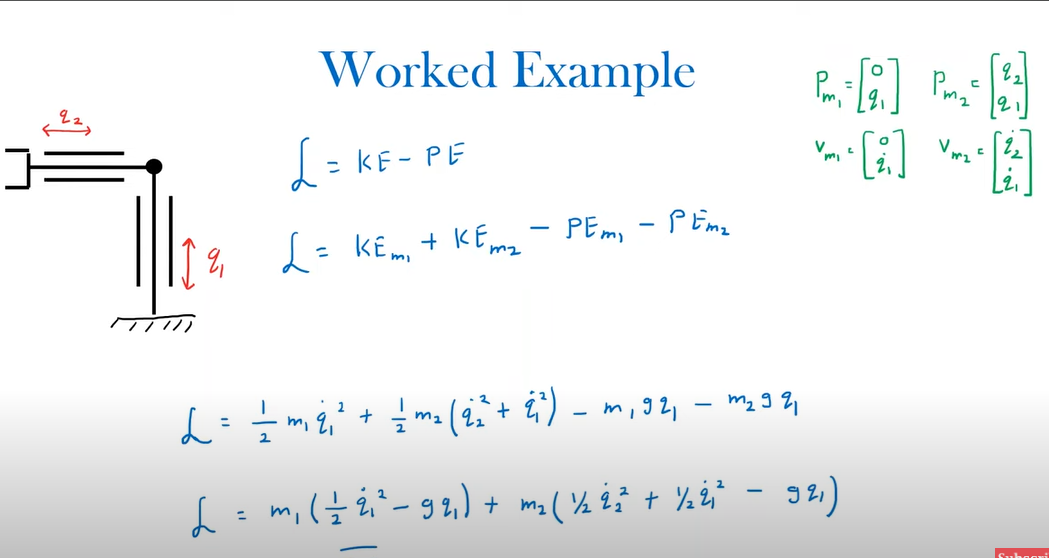
\includegraphics[width=10cm]{part3_lagrange.png}\\
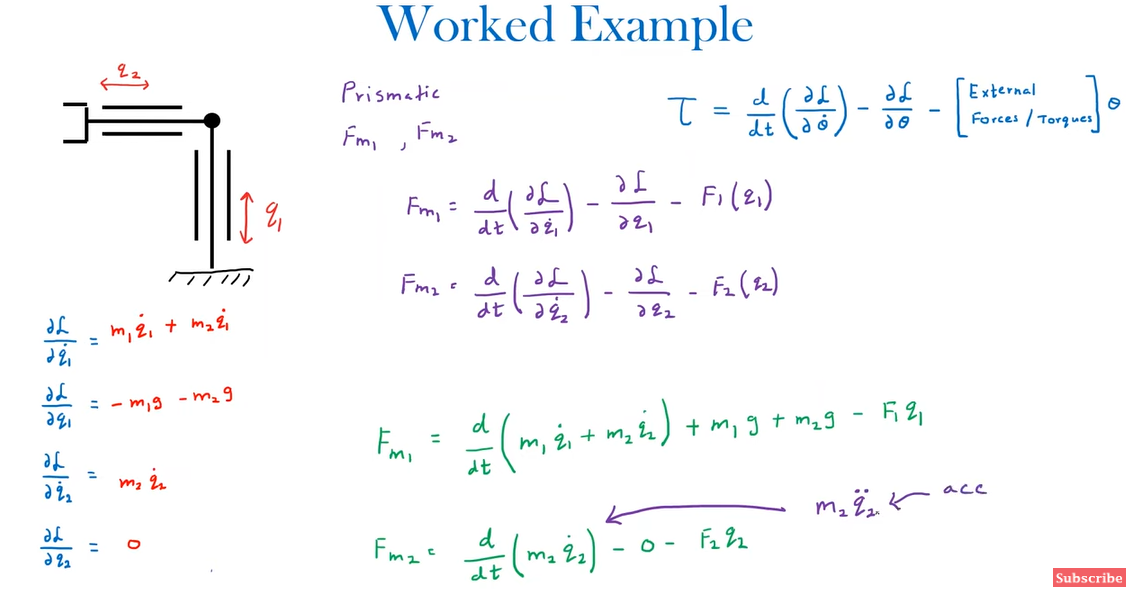
\includegraphics[width=10cm]{part4_lagrange.png}

\section{Trajectory Planning and Generation}
\textbf{Trajectory:} Time history of position, velocity and acceleration for each DOF.\\
\begin{itemize}
    \item Run time
    \item Path update rate (60-2000hz)
    \item You also want smooth motion(minimze wear and tear)
    \item \textbf{Via points:} auxilary/intermediate points between initial and final positions
    \item Optimization problem because there are many ways to potentially go from initial to final
\end{itemize}

\textbf{Path Generation Methods}
\begin{itemize}
    \item Joint Space Schemes $\rightarrow$ using function of joint angles(in terms of $\theta$),  each via point(including final and initial) is converted to a set of joint angles using inverse kinematics
    \item Cartesian Schemes $\rightarrow$ directly uses the position and orientation of the robot frames along with the path points as specified by the user to generate the trajectory.
\end{itemize}
In general, joint space schemes are easier to use and compute. This is because cartesian schemes require inverse kinematics to be used at every single point along the path, in the path update. So higher computational burden on the robot. 

\subsection{Joint Space Schemes}
Is split into two sub methods:
\begin{itemize}
    \item Cubic Polynomials(can be even higher order)
    \item Parabolic Blends
\end{itemize}

\subsection{Cubic Polynomials}
The idea here is to find an equation(3rd degree polynomial) that satisfies the following constraints:\\
\begin{itemize}
    \item $\theta(t_0)=\theta_0$ aka the initial position at time 0 is the initial position of the robot
    \item $\dot{\theta(0)}=0$ aka the derivative of the initial postion has velocity 0
    \item $\theta(t_f) = \theta_f$ the final position at time f, is at the intended final position
\end{itemize}
To model a polynomial with 4 constraints you need at least a 3rd degree polynomial. If you add via points, then you can increase the degree of the polynomial by adding additional constraints. \\\\
\textbf{Form of functions:}\\
\begin{itemize}
    \item $\theta(t)=a_0+a_1t+a_2t^2+a_3t^3$ Position
    \item $\dot{\theta(t)}=a_1+2a_2t+3a_3t^2$ Velocity
    \item $\ddot{\theta(t)}=2a_2+6a_3t$ Acceleration
\end{itemize}
\textbf{Example:}\\
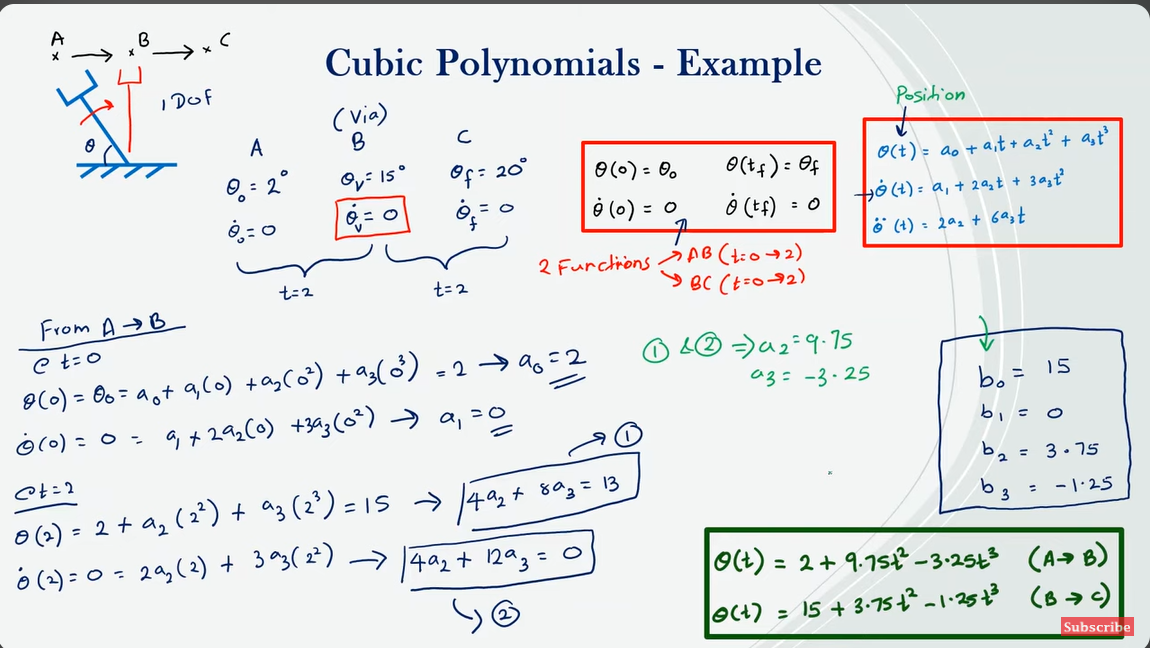
\includegraphics[width=10cm]{cubic_polynomial_example.png}

\subsection{Parabolic Blends}
To solve discontinuous velocities, we use parabolic blends.\\
\textbf{Explanation:}\\
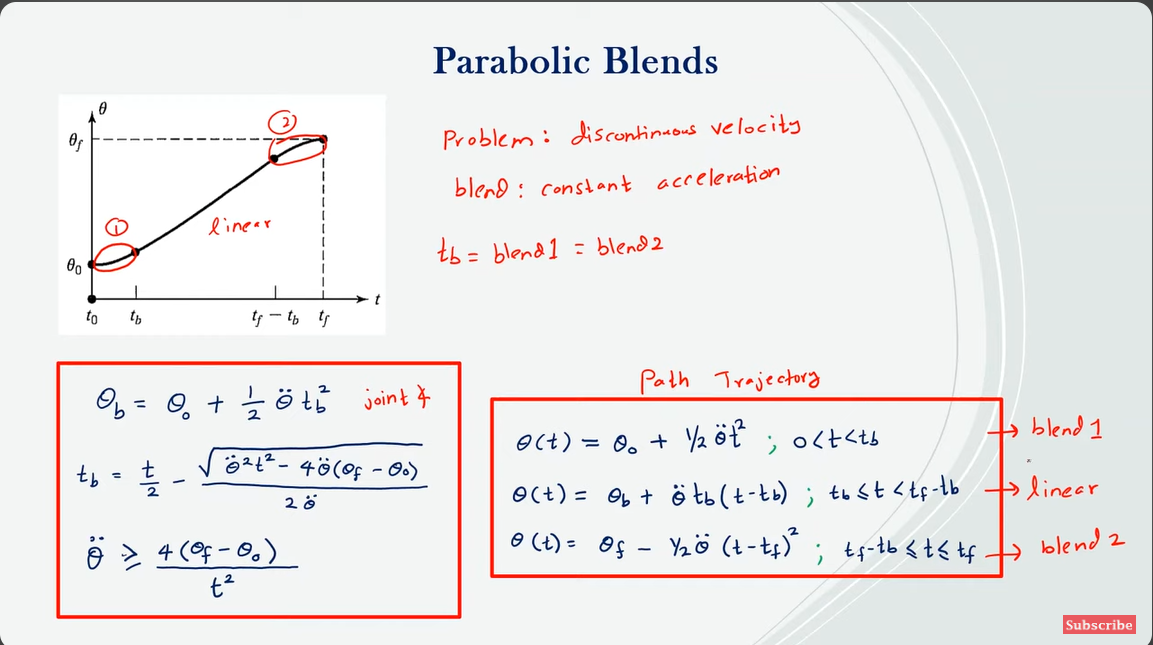
\includegraphics[width=10cm]{parabolic_explanation.png}\\
\textbf{Example:}\\
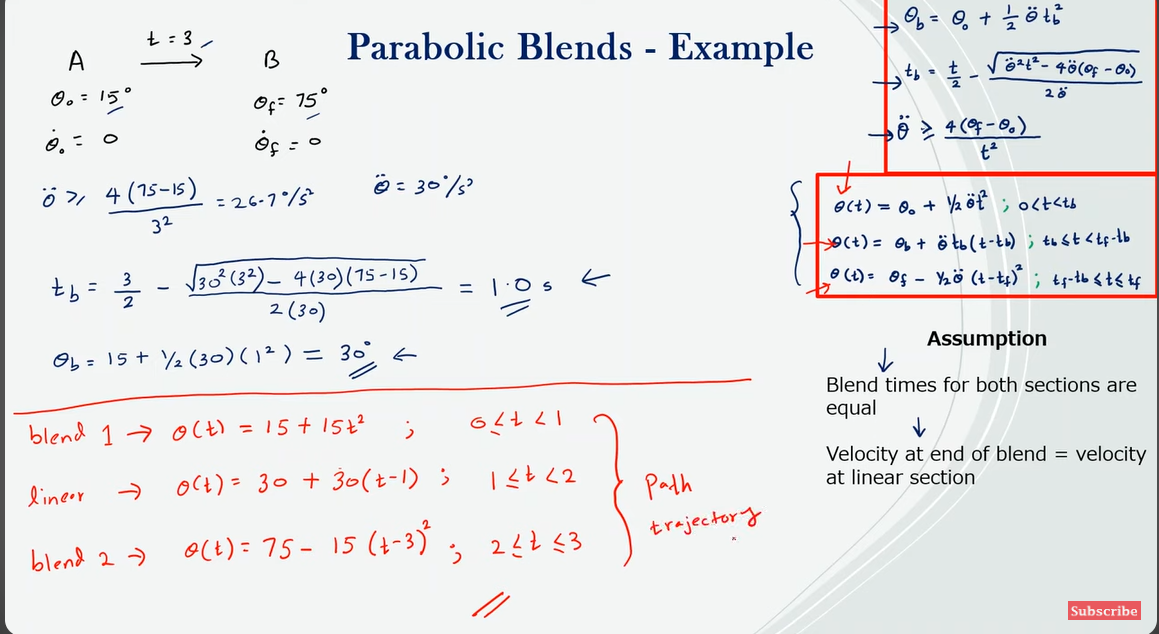
\includegraphics[width=10cm]{parabolic_example.png}

%\section{LIE Algebra}

\section{Credit}
These are my notes from the robotics playlist youtube channel @thatsengineering5235, all of the external images used are examples from their videos. 
\end{document}
